\documentclass[12pt]{article}

\usepackage[letterpaper, margin=1in]{geometry}
\usepackage{times}
\usepackage{setspace}
\usepackage{lipsum}
\usepackage{graphicx}
\usepackage{float}

\title{Transfer Learning for American Sign Language Dataset}
\author{Josh Hills - 101142996\\COMP 4107\\Professor Holden}
\date{\today}

\begin{document}
\maketitle
\newpage
\subsection*{Introduction}
\quad
Transfer learning is a machine learning technique that allows a pre-trained neural network model to be fine-tuned on a smaller, task-specific dataset. The use of transfer learning has become 
increasingly prevalent in the field of deep learning, specifically in image recognition, natural language processing, and reinforcement learning. The purpose of this final project is to investigate
the effectiveness of transfer learning when applied to the task of classifying ASL hand gestures. There is an abundance of great research studying transfer learning, such as Weiss et al. (2016). We will
build on these foundational studies and surveys to learn how transfer learning can be applied to our specific problem. Transfer learning has lots of potential for reducing computation required in
deep learning projects, making time for computation a topic of this study. The primary goal of this paper is to evaluate the effectiveness of transfer learning, comparing the performance of the fine-tuned
pre-trained models from a model we make without transfer learning. I find transfer learning particularly interesting as an individual, sometimes we feel limited to projects we can do alone because of the 
limited amount of data an individual can collect, computation power an individual has access to. Using transfer learning we can leverage research of others and in a literal sense 
open up the number of possibilities that your average person has in research and development. 

\subsection*{Methods}
\quad
For the training of the model, convolutional neural networks (CNNs) will be used. While we will be testing multiple pre-trained neural networks, we will only be talking about the architecture of VGG16, and how
it is modified to solve our new task. First lets talk about how image classification works. Pretending that image classification is a black box for a second, the task of image classification is given
an input image x, output a single class that the image most likely falls into. For example, if we consider a model trained on the popular ImageNet dataset, given an image the model tries to guess which of the
1000 classes the image most likely is. Enter the VGG16 model for the ImageNet dataset. \\
\begin{figure}[H]
    \centering
    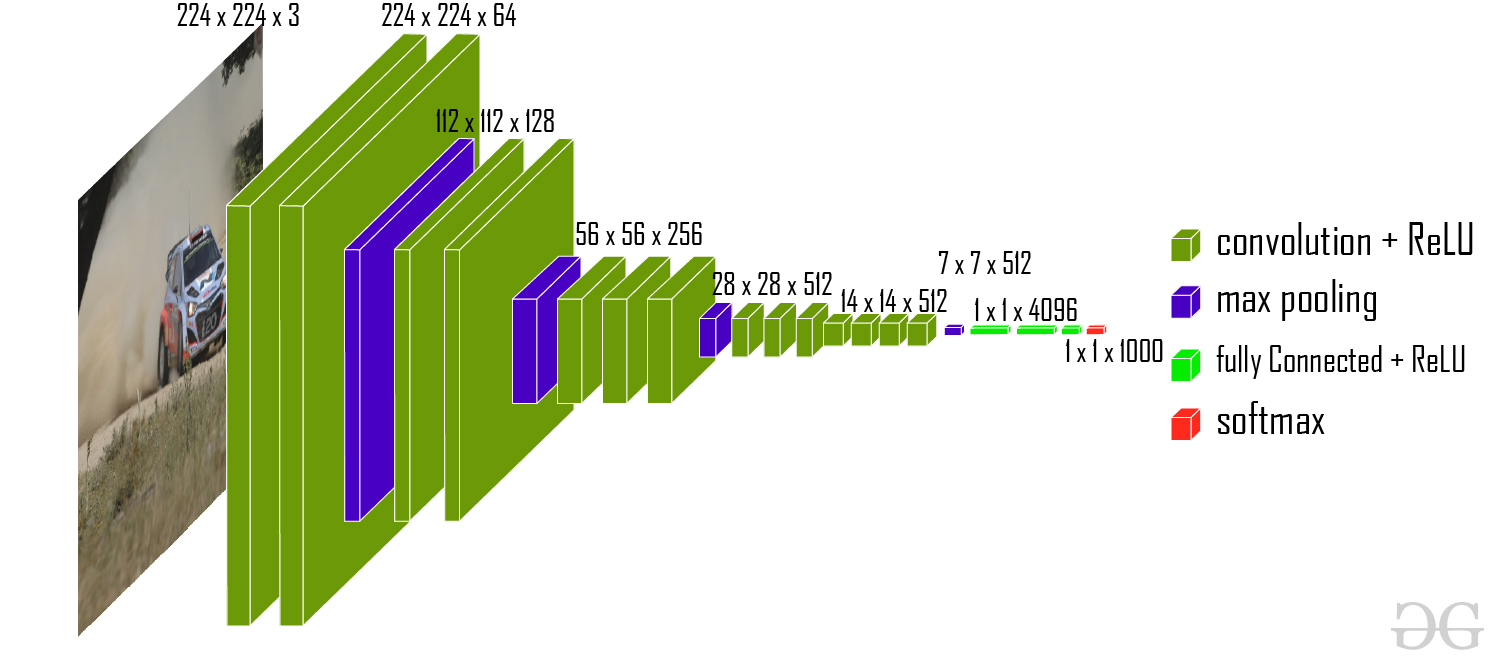
\includegraphics[scale=0.25]{images/vgg-architechture.jpg}\\
    https://www.geeksforgeeks.org/vgg-16-cnn-model/
\end{figure}
The above shows the network architecture of the VGG16 model which was trained using the ImageNet dataset. This dataset contains 224x224 images with RGB channels, this gives us an input tensor of 224x224x3.
As this is an example of a CNN, we then see a series of convolution layers using a ReLU activation followed by max pooling layers. This architecture shows 5 convolution/pooling operations, in some cases there are 2 convolutions before 
pooling and sometimes 3 convolutions. After this series of operations we have a 7x7x512 feature map. Then, this output is flattened to make it a 1x25088 feature vector. Following this is 3 
fully connected layers, finally giving us a 1x1000 output. Using the softmax, we get the class predicted for our image. We can imagine the final output vector as $\hat{y} = [\hat{y_0}; \hat{y_1}; \hat{y_2}; ... ; \hat{y_{999}}]$, which contains scores
of each class, taking the $softmax(\hat{y})$ gives us the probability of each class. The max of the softmax is the predicted class. So why is this useful to us? How can we use this model to predict
the classes for the ASL dataset? Essentially, the reason this is so useful, as I mentioned above we create a feature map before our actual classification. The features in this map can be useful for a new model,
to think about our specific example. ImageNet has a load of classes [2], we can assume by VGG16's very high accuracy that it has a good understanding of the natural world, and thus maybe understands what a hand looks like, meaning 
where a hand is in the image is not a feature that our fine-tuned model will have to learn. Compared to a model that we train from scratch, will have to use it's limited dataset to figure out more simple features. We cut off
the flattening and then dense layers at the end of the neural network and create our own, we then fit the model using the ASL images and are given a new model. \\


This study uses two main datasets, one directly and one indirectly. While we do not actually use the dataset the ImageNet dataset, I think it is still important to explain it here to gain a full grasp of 
transfer learning's value. ImageNet is a dataset consisting of approximately 14 million images that each belong to one of 1000 classes [3]. ImageNet was first created to establish a good benchmark test
to be used for object categorization. Researchers work hard to develop new and better algorithms to organize and annotate video and image data, better tools require better data to train their algorithms on.
We can imagine how a model build using ImageNet can be used to categorize our pictures, think about this as the technology that allows us to search all the pictures on our iPhones for those containing a cat. 



% [2] https://deeplearning.cms.waikato.ac.nz/user-guide/class-maps/IMAGENET/
% [3] https://www.image-net.org/about.php
% [4] https://www.kaggle.com/code/abdul390/asl-recognition-with-convolutional-neural-networks







\end{document}